\documentclass[xcolor=table]{beamer}
\usepackage{fontspec}
\usepackage{natbib}
\usepackage{gb4e} 
\usepackage[table]{xcolor}
\usepackage{booktabs} 
%\usepackage{color}
\usepackage{graphicx}
\usepackage{tikz}
\usetikzlibrary{trees}

% \setmainfont[Mapping=tex-text]{Charis SIL}
\let\sfdefault\rmdefault
%\newcommand{\racine}[1]{\begin{math}\sqrt{#1}\end{math}} 
\newfontfamily\phon[Mapping=tex-text,Ligatures=Common,Scale=MatchLowercase,FakeSlant=0.3]{Charis SIL} 
\newcommand{\ipa}[1]{{\phon \mbox{#1}}} %API tjs en italique
\newcommand{\grise}[1]{\cellcolor{lightgray}\textbf{#1}} 
\newcommand{\ra}{$\Sigma_1$} 
\newcommand{\rc}{$\Sigma_3$} 
\newcommand{\ro}{$\Sigma$} 
 \begin{document}

 \title{From ergative to index of comparison: multiple reanalyses and polyfunctionality}
 \author{Guillaume Jacques}
 \maketitle
 
  \begin{frame} 
 \frametitle{Japhug and other Rgyalrongic languages} 
 \begin{figure}[H]
\centering
\includegraphics[height=30mm]{carte.JPG}
\end{figure}
 
Unlike most languages of the Sino-Tibetan family: 
 
 \begin{enumerate}[<+->]
 \item Polysynthetic (polypersonal agreement, incorporation), complex templatic morphology (\citealt{jacques13harmonization})
  \item Direct-inverse agreement system (\citealt{jacques10inverse})
 \item Complex morphophonological alternations
 \item Very rich voice morphology (antipasstive, passive, causative, applicative etc)
 \item Complex consonant clusters (for instance \ipa{lɟɣaʁ} `put on')
 \item Strict accusative AND ergative pivots in various domains of the morphosyntax.
 \item Barely any non-trivial morphosyntactic feature in common with Chinese or Burmese.
 \end{enumerate}
  
  \end{frame}   


  \begin{frame} 
 \frametitle{Grammaticalization in Japhug} 

A considerable part of the rich morphology found in Japhug is relatively recent and its origin still relatively transparent.

 \begin{enumerate}[<+->]
 \item bare nominalization + denominal $\Rightarrow$  Voice derivations (in particular antipassive and applicative, see \citealt{jacques14antipassive})
 \item Noun-Verb synthetic compounds + Denominal $\Rightarrow$  Incorporation (\citealt{jacques12incorp})
   \item S/A Nominalizing prefix $\Rightarrow$  Generic person marking and 2$\rightarrow$1 portmanteau prefix
   \item second person + passive $\Rightarrow$ 1$\rightarrow$2 portmanteau prefix
	\item Garden variety changes:
 \begin{enumerate}	
 \item Orientational prefixes $\Rightarrow$  various TAM markers (\citealt{jackson07irrealis, lin11direction, jacques14linking})
 \item Motion verbs $\Rightarrow$ Associated motion (\citealt{jacques13harmonization})
  \item etc...
  \end{enumerate}
 \end{enumerate}

  \end{frame}   



  \begin{frame} 
 \frametitle{Areal context} 

 \begin{enumerate}[<+->]
 \item Considerable impact of various dialects of Tibetan on the Japhug lexicon.
 \item Tibetan influence on the evidential system
 \item Some linkers are of Tibetan origin (for instance \ipa{nɤ} in the protasis of conditionals).
 \item The ergative \ipa{kɯ} and the genitive \ipa{ɣɯ} have been recently borrowed from Amdo Tibetan.
 \item Some recent lexical influence from Sichuan Chinese.
 \end{enumerate}

  \end{frame}   


  \begin{frame} 
 \frametitle{The ergative/ instrumental} 

\begin{exe}
\ex \label{ex:erg}
\gll [\ipa{tɤ-tɕɯ}  	\ipa{nɯ}]  	\ipa{\textbf{kɯ}} 	\ipa{χsɤr}  	\ipa{qaɕpa}  	\ipa{nɯ}  	\ipa{cʰɤ-mqlaʁ}   \\
\textsc{indef.poss}-boy \textsc{dem} \textsc{erg} gold frog \textsc{dem} \textsc{evd}-swallow \\
\glt `The boy swallowed the golden frog.' (Nyima Wodzer.1, 131)
\end{exe}


 \begin{exe}
\ex \label{ex:instr2}
\gll [\ipa{nɯ-mtsioʁ}   	\ipa{nɯ}]   	\ipa{\textbf{kɯ}}   	\ipa{lu-sɯ-lɣa-nɯ}   	\ipa{qʰe,}   	\ipa{tɤtsoʁ}   	\ipa{lu-nɯ-tɕɤt-nɯ}   	\ipa{ɲɯ-ŋgrɤl}   	\ipa{kʰi}        \\
\textsc{3pl.poss}-beak \textsc{dem} \textsc{erg/instr} \textsc{ipfv-caus}-dig-\textsc{pl} \textsc{lnk} potentilla.anserina \textsc{ipfv-auto}-take.out-\textsc{pl} \textsc{ipfv}-be.usually.the.case \textsc{hearsay} \\
\glt  `(The wild geese) dig (the ground) with their beaks, and they take out Potentilla anserina roots.' (Wild Geese 28)
\end{exe}
  \end{frame}   

%
  \begin{frame} 
 \frametitle{The ergative/ instrumental} 
  \framesubtitle{Comparative construction} 
 Also used on the comparee (NOT the standard!) in the comparative construction:
 
 
 \begin{exe}
\ex \label{ex:comp1}
\gll  \ipa{ɯ-ʁi}   	\ipa{sɤz}   	[\ipa{ɯ-pi}   	\ipa{nɯ}]   	\ipa{\textbf{kɯ}}   	\ipa{mpɕɤr}     \\
\textsc{3sg.poss}-younger.sibling \textsc{comparative} \textsc{3sg.poss}-elder.sibling \textsc{dem} \textsc{erg?}  \textsc{n.pst:}be.beautiful \\
\glt `The elder one is more beautiful than the young one.' (elicited)
\end{exe}

\begin{exe}
\ex \label{ex:comp.eng}
\gll  John is more intelligent than Paul \\
\textsc{comparee} { } \textsc{index} \textsc{parameter} \textsc{mark} \textsc{standard}  \\
\end{exe}
  \end{frame}   

  \begin{frame} 
 \frametitle{The ergative/ instrumental} 
  \framesubtitle{Comparative tropative construction}

 \begin{exe}
\ex \label{ex:kWkWmWm}
\gll  \ipa{tɕe}   [\ipa{tʰoŋ-raʁ}   	\ipa{nɯ}]   	\ipa{kɯ}   	\ipa{kɯ-mɯm}   	\ipa{tu-sɯpa-nɯ}   	\ipa{ŋu}   \\
\textsc{lnk} bucket.alcohol \textsc{dem} \textsc{erg} \textsc{inf:stat}-be.tasty \textsc{ipfv}-consider-\textsc{pl} be:\textsc{fact} \\
\glt `They consider  bucket alcohol to be tastier (than the pan-alcohol).' (Distilled alcohol, 15)
\end{exe}

\begin{exe}
\ex \label{ex:nAmWm}
\gll  [\ipa{tʰoŋraʁ} 	\ipa{nɯ}] 	\ipa{kɯ} 	\ipa{ɲɯ-nɤ-mɯm-nɯ} \\
 bucket.alcohol \textsc{dem} \textsc{erg}  \textsc{testim-trop}-be.tasty-\textsc{pl} \\
 \glt `They consider  bucket alcohol to be tastier (than the pan-alcohol).'  (elicited).
\end{exe}

  \end{frame}   
  
  \begin{frame} 
 \frametitle{The ergative/ instrumental} 
 \framesubtitle{Relativization} 
 

\begin{enumerate}
\item A: \ipa{ɯ-kɯ--} participle
\item instrument: \ipa{sɤ--} participle
\item comparee: \ipa{kɯ--} participle
\end{enumerate}
 
 
\begin{exe}
\ex \label{ex:pjWkAm}
\gll
[\ipa{ɯʑo}  	\ipa{sɤz}  	\ipa{kɯ-wxti}]  	\ipa{rɯdaʁ}  	\ipa{ra}  	\ipa{kɯnɤ}  	\ipa{pjɯ-kɤm}  	\ipa{ɕti}  \\
it \textsc{comp} \textsc{nmlz}:S-big animal \textsc{pl} also \textsc{ipfv}-prevail[III] \textsc{n.pst:}be:\textsc{assert} \\
\glt `It also prevails over animals that are bigger than itself.' (The lion, 23)
  \end{exe}
\end{frame}   


  \begin{frame} 
 \frametitle{The ergative/ instrumental} 


Are these two \ipa{kɯ} markers historically related?

\end{frame}   


  \begin{frame} 
 \frametitle{Other constructions} 
 \framesubtitle{Cause} 

\begin{exe}
\ex \label{ex:sWmWzdWG.kW}
\gll 
[\ipa{sɯmɯzdɯɣ}]  	\ipa{kɯ}  	\ipa{ɕɤr}  	\ipa{ɯ-ʑɯβ}  	\ipa{mucin}  	\ipa{mɯ-pɯ-ɣe}  	\ipa{ɲɯ-ŋu.}  	 \\
worry  \textsc{erg/instr} night \textsc{3sg.poss}-sleep at.all \textsc{neg-pfv}-come[II] \textsc{testim}-be \\
\glt `As she was worried, she could not get any sleep for the whole night.' (Slobdpon, 174)
\end{exe}



\begin{exe}
\ex \label{ex:WxCAt.kW}
\gll
[\ipa{tɯ-mŋɤm} 	\ipa{ɯ-xɕɤt}] 	\ipa{kɯ} 	\ipa{aʑo} 	\ipa{nɯ} 	\ipa{a-ku} 	\ipa{ɕɤrɯ} 	\ipa{pjɤ-ɣɤtsɯr} 	\ipa{ɲɯ-ŋu} 	\ipa{nɯ-sɯso-t-a.} 	\\
\textsc{nmlz:action}-hurt \textsc{3sg.poss}-strength \textsc{erg/instr} \textsc{1sg} \textsc{dem} \textsc{1sg.poss}-head bone \textsc{evd}-have.a.crack \textsc{testim}-be \textsc{pfv}-think-\textsc{pst-1sg} \\
\glt `Because to the pain, I felt as though my skull had cracked.' (Headache, 77)
  \end{exe}

\end{frame}   

  \begin{frame} 
 \frametitle{Other constructions} 
 \framesubtitle{Manner (infinitival clause)} 
\begin{exe}
\ex \label{ex:mAkApa.kW}
\gll
\ipa{tɕe}   	\ipa{ɯ-ŋgɯ}   	\ipa{nɯ} \ipa{tɕu}   	\ipa{paʁndza}   	\ipa{ɲɤ-raʁ}   	\ipa{tɕe,}   	\ipa{tɕendɤre}   	[<dian>   	<guan>   	\ipa{mɤ-kɤ-βzu}] 	\ipa{\textbf{kɯ}}   	[\ipa{mɤ-kɤ-pa}]   	\ipa{\textbf{kɯ}}   	\ipa{ɯ-jaʁ}   	\ipa{lo-tsɯm}\\
\textsc{lnk} \textsc{3sg}-inside \textsc{dem} \textsc{loc} pig.fodder \textsc{evd}-be.stuck \textsc{lnk}
\textsc{lnk} electricity turn.off \textsc{neg-inf}-make \textsc{erg}  \textsc{neg-inf}-close \textsc{erg}  \textsc{3sg.poss}-hand \textsc{evd:upstream}-take\\
\glt `Some pig fodder got stuck inside (the machine) he put his hand into it without turning it off,' (Relatives, 372-3)
\end{exe} 
\end{frame}   

  \begin{frame} 
 \frametitle{Other constructions} 
 \framesubtitle{Manner (Finite clause)} 
 \begin{exe}
\ex \label{ex:mWjfse.kW}
\gll
\ipa{ri} 	\ipa{ɯ-jwaʁ} 	\ipa{nɯnɯ} 	[\ipa{kɯmaʁ} 	\ipa{ɕɤɣ} 	\ipa{nɯ} \ipa{ra} 	\ipa{mɯ́j-fse}] 	\ipa{\textbf{kɯ}} 	\ipa{ɲɯ-ɤrʁɯrʁu} 	\ipa{ʑo} 	\ipa{qʰe} 	\ipa{ɲɯ-ɤndɯndo} 	\ipa{ʑo.} \\
\textsc{lnk} \textsc{3sg.poss}-leaf \textsc{dem} other juniper \textsc{dem} \textsc{pl} \textsc{neg:testim}-be.like \textsc{erg?} \textsc{testim}-be.wrinkled \textsc{emph} \textsc{lnk}  \textsc{testim}-be.clustered.together \textsc{emph} \\
\glt `Its leaves differ from other junipers in that they are wrinkled and clustered together.' (Ephedra, 71)
 \end{exe}

\end{frame}   
 
  \begin{frame} 
 \frametitle{Other constructions} 
 \framesubtitle{Empatic adversative} 

 \begin{exe} 
 \ex \label{ex:YWmaR.kW}
\gll [\ipa{tɯrgi} 	\ipa{kɯ-fse} 	\ipa{ɯ-stu} 	\ipa{tu-ɕe} 	\ipa{ɲɯ-maʁ}] 	\ipa{kɯ,} \ipa{aʁɤndɯndɤt} 	\ipa{ɯ-rtaʁ} 	\ipa{ɲɯ-ɬoʁ} 	\ipa{ɲɯ-ŋu} 	\ipa{tɕe,} 
\\
fir \textsc{inf:stat}-be.like \textsc{3sg.poss}-straight \textsc{ipfv:up}-go \textsc{testim}-not.be \textsc{erg}? everywhere \textsc{3sg.poss}-branch \textsc{testim}-come.out \textsc{testim}-be \textsc{lnk} \\ 
\glt `It does not grow straight like the fir, on the contrary, its branches spread out in all directions.'  
(maldo, 54)
 \end{exe}  
 
\end{frame}     


  \begin{frame} 
 \frametitle{Other constructions} 
 \framesubtitle{Degree construction (monoclausal)} 
\begin{exe}
\ex \label{ex:YWsWxtCur}
\gll 
\ipa{mtɕʰi}  	\ipa{ɯ-mat}  	\ipa{rca}  	\ipa{ɯ-tɯ-tɕur}  	\ipa{saχaʁ.}  	   \\
sea.buckthorn \textsc{3sg.poss}-fruit \textsc{dem} \textsc{3sg-nmlz:degree}-be.sour \textsc{n.pst}:be.extremely   \\
\glt `The fruit of the sea-buckthorn is very sour,' (Sea-buckthorn, 65)
\end{exe}
\end{frame}     

  \begin{frame} 
 \frametitle{Other constructions} 
 \framesubtitle{Degree construction (biclausal)} 
\begin{exe}
\ex \label{ex:YWsWxtCur2}
\gll 
 	[\ipa{ɯ-tɯ-tɕur}]  	\ipa{\textbf{kɯ}}  	[\ipa{tɯ-kɯr}  	\ipa{ɯ-ŋgɯ}  	\ipa{lú-wɣ-rku}  	\ipa{qʰe}  	\ipa{maka}  	\ipa{ɲɯ-sɯ-ɤmɯzɣɯt}  	\ipa{qʰe,}  	\ipa{tɯ-pʰoŋbu}  	\ipa{ra}  	\ipa{kɯnɤ}  	\ipa{ɲɯ-sɯx-tɕur}  	\ipa{kɯ-fse}  	\ipa{ɕti}]  \\
  \textsc{3sg-nmlz:degree}-be.sour \textsc{erg?} \textsc{indef:poss}-mouth \textsc{3sg}-inside \textsc{ipfv:upstream-inv}-put.in \textsc{lnk} at.all \textsc{ipfv-caus}-be.evenly.distributed \textsc{lnk} \textsc{indef:poss}-body \textsc{pl} also \textsc{ipfv-caus}-be.sour \textsc{nmlz:S/A}-be.like be:\textsc{affirm}:\textsc{fact} \\
\glt `(The fruit of the sea-buckthorn) is so sour that when one puts it in one's mouth, it makes it completely (sour), and it is as if one's (whole) body became sour.' (Sea-buckthorn, 66)
\end{exe}
\end{frame}     


  \begin{frame} 
 \frametitle{Other constructions} 
 \framesubtitle{Degree construction (biclausal)} 

 \begin{exe}
\ex \label{ex:WtWmbjom}
\gll 
\ipa{tɯ-ci}  	\ipa{ɯ-ɣmbɤj}  	\ipa{nɯ}  	\ipa{tɕu,}  	  	\ipa{tɤ-rtsa}  	\ipa{kɯ-xtɕɯ-xtɕi}  	\ipa{nɯ}  	\ipa{χanɯni}  	\ipa{ju-ɕe}  	\ipa{ɲɯ-ŋu}  	\ipa{ma}  	\ipa{nɯ}  	\ipa{ma}  	\ipa{kɯ-saχsɤl}  	\ipa{maŋe,}  	[\ipa{ɯ-tɯ-mbjom}]  	\ipa{\textbf{kɯ}.}  \\
\textsc{indef.poss}-water \textsc{3sg.poss}-side \textsc{dem} \textsc{loc} \textsc{indef.poss}-wave \textsc{nmlz:S/A-redp}-be.small \textsc{dem} a.little \textsc{ipfv}-go \textsc{testim}-be apart.from \textsc{dem} apart.from   \textsc{nmlz:S/A}-be.clear not.exist:\textsc{testim} \textsc{3sg-nmlz:degree}-be.quick \textsc{erg?} \\
\glt `(When it dives into the water), it is so quick that one can only see little ripples near the shore.'
 (Kingfisher, 54)
\end{exe}

\end{frame}     


  \begin{frame} 
 \frametitle{Pathway} 
 Pathway 1:
\begin{enumerate}
\item Instrumental $\Rightarrow$ Cause $\Rightarrow$ Manner (already in Tibetan)
\item Manner  $\Rightarrow$ Adversative
\item Adversative $\Rightarrow$ Index of comparison
\end{enumerate}

Pathway 2:
\begin{enumerate}
\item Instrumental $\Rightarrow$ Cause $\Rightarrow$ Manner 
\item Manner  $\Rightarrow$ Degree Construction
\item Degree $\Rightarrow$ Index of comparison
\end{enumerate}
\end{frame}     

  \begin{frame} 
 \frametitle{Adversative $\Rightarrow$ Index of comparison}
  \framesubtitle{Stage one}
\begin{exe}
  \ex  \label{ex:mAYaR.kW}  
  \gll 
  \ipa{mtsʰalɤɲaʁ} 	\ipa{nɯ} 	\ipa{ɯ-mdoʁ} 	\ipa{ɲaʁ} 	\ipa{tsa} 	\ipa{mtsʰalɤɣrum} 	\ipa{nɯnɯ} 	\ipa{tɕe,} 	[\ipa{nɯ} \ipa{stʰɯci} 	\ipa{mɤ-ɲaʁ}] 	\ipa{kɯ}   	\ipa{aqarŋɯrŋe} 	\ipa{kɯ-fse} 	\\
  black.nettle \textsc{dem} \textsc{3sg.poss}-colour be.black:\textsc{fact} a.little   white.nettle \textsc{dem} \textsc{lnk} \textsc{dem} as.much neg-be.black:\textsc{fact}  \textsc{erg?} be.yellowish:\textsc{fact} \textsc{inf:stat}-be.like \\
  \glt `The colour of the black nettle is black, and the white nettle, it is not as  black but rather yellowish.'   (Nettle 21-23)
        \end{exe} 
        
\begin{exe}
  \ex  \label{ex:mWYArtWm.kW}  
  \gll      
\ipa{ɯ-jwaʁ} 	\ipa{nɯ} \ipa{ra} 	\ipa{iʑora} 	\ipa{ji-paχɕi} 	[\ipa{stʰɯci} 	\ipa{mɯ-ɲɯ-ɤrtɯm}] 	\ipa{kɯ} 	\ipa{ɲɯ-rɲɟi} 	\ipa{tsa.} \\
\textsc{3sg.poss}-leaf \textsc{dem} \textsc{pl} \textsc{1pl} \textsc{1pl.poss}-apple so.much \textsc{neg-testim}-be.round \textsc{erg?} \textsc{testim}-be.long little \\
\glt `Its leaves  are not as round as those of the apple of our (country), but are rather a little long.'
(Apple, 49)
\end{exe} 

\end{frame}     




  \begin{frame} 
 \frametitle{Adversative $\Rightarrow$ Index of comparison}
  \framesubtitle{Stage two}
 \begin{exe}
  \ex  \label{ex:mWYArtWm.kW3}  
  \gll      
[\ipa{ɯ-jwaʁ} 	\ipa{nɯ}   \ipa{ra}] 	\ipa{kɯ} 	\ipa{ɲɯ-rɲɟi} 	\ipa{tsa.} \\
\textsc{3sg.poss}-leaf \textsc{dem} \textsc{pl}   \textsc{erg?} \textsc{testim}-be.long little \\
\glt *`Its leaves are rather a little long'  $\rightarrow$  `Its leaves are a little longer.'
(Adapted from \ref{ex:mWYArtWm.kW})
          \end{exe} 
\end{frame}     


  \begin{frame} 
 \frametitle{Adversative $\Rightarrow$ Index of comparison}
\begin{enumerate} 
\item 
\begin{enumerate} 
\item S [not.long] \ipa{kɯ} long 
\item `S is rather long than not long'
\end{enumerate} 
\item Elision of the verb phrase in the adversative construction  and reanalysis of the S as being under the syntactic scope of \ipa{kɯ}
\begin{enumerate} 
\item{} [S] \ipa{kɯ} long  
\item *`S is rather long' (not attested)
\end{enumerate} 
\item Semantic change to a comparative construction (without overt standard of comparison)
\begin{enumerate} 
\item{} [S] \ipa{kɯ} long  
\item `S is longer'  
\end{enumerate} 
\item Introduction of the standard (S_2)
\begin{enumerate} 
\item{} S_2 \ipa{sɤz} [S] \ipa{kɯ} long  
\item  `S is longer than S_2'
\end{enumerate} 
\item Generalization to tropative construction
\begin{enumerate} 
\item{}  [S] \ipa{kɯ} long  consider  
\item  `consider S to be be longer'
\end{enumerate}  
\end{enumerate}
\end{frame}     
  
 \begin{frame} 
 \frametitle{Summary}

  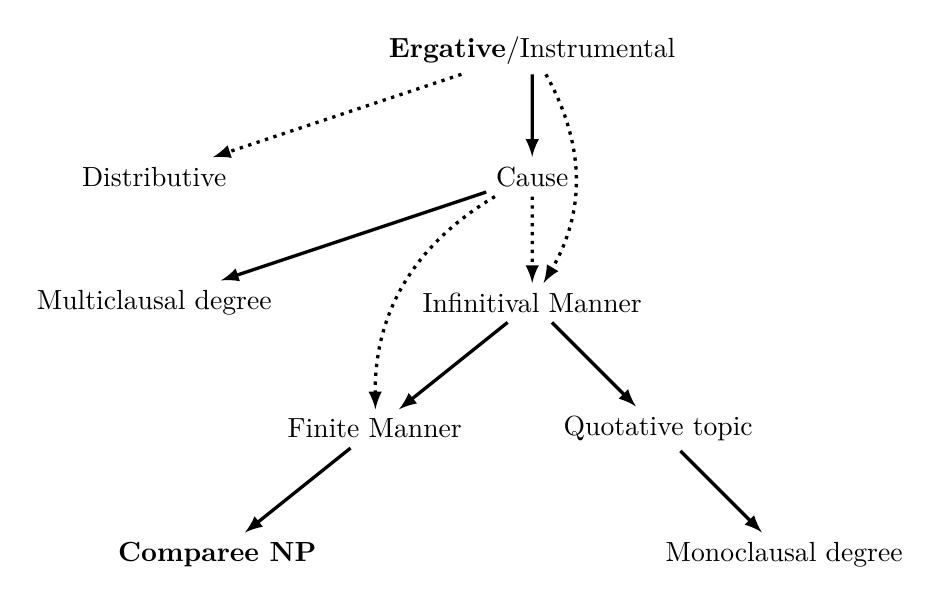
\begin{tikzpicture}[scale=0.80]
  \node (A) at (4,1) {\textbf{Ergative}/Instrumental};
   \node (B) at (-2,-1) {Distributive};
    \node (C) at (4,-1) {Cause};
        \node (D) at (-2,-3)  {Multiclausal degree};
    \node (E) at (4,-3) {Infinitival Manner}; 
       \node (F) at (1.5,-5)  {Finite Manner};%\\ Adversative};
        \node (G) at (6,-5) {Quotative topic}; 
             \node (H) at (-1,-7)  {\textbf{Comparee NP}};
             \node (I) at (8,-7) {Monoclausal degree}; 
  %  \node (J) at (-0.5,-9) {\textbf{Comparee NP}};
    
    
\tikzstyle{peutetre}=[->,dotted,very thick,>=latex]
\tikzstyle{sur}=[->,very thick,>=latex]
\draw[peutetre] (A)--(B);
\draw[sur] (A)--(C);
\draw[sur] (C)--(D);
\draw[peutetre] (C)--(E);
\draw[peutetre] (A) to[bend left] (E);
\draw[sur] (E)--(F);
\draw[sur] (E)--(G);
\draw[sur] (F)--(H);
\draw[sur] (G)--(I);
%\draw[sur] (H)--(J);
\draw[peutetre] (C) to[bend right] (F);
\end{tikzpicture}
 \end{frame}


 \begin{frame} 
 \frametitle{References}
 \tiny
 \bibliographystyle{unified}
\bibliography{bibliogj}
 \end{frame}
\end{document}